\section{Actividad No 07 – Funciones de Agrupaci\'on} 
		
\begin{enumerate}[1.]
	\item El departamento de Recursos Humanos requiere un reporte que muestre el máximo, el mínimo, la suma y el promedio de los salarios de todos los empleados, Etiquetar esta columnas como Máximo, Mínimo, Suma y Promedio respectivamente, Redondear estos valores a enteros sin decimales.
	\\
	\\SELECT ROUND(MAX(salary),0) AS "Maximo" , ROUND(MIN(salary),0) AS "Minimo", ROUND(SUM(salary),0) AS "Sumatoria", ROUND(AVG(salary),0) AS "Promedio"
	\\FROM employees;
    	\begin{center}
	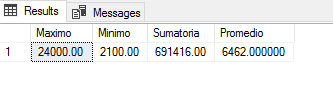
\includegraphics[width=5cm]{./Imagenes/a7a1} 
	\end{center}

	\item Modificar la consulta anterior para mostrar el máximo, mínimo, suma y promedio de los salarios por cada Puesto de trabajo. 
	\item Realizar un reporte que muestre la cantidad de empleados por Puesto de trabajo. Con la opción de que el usuario pueda ingresar todos los puestos o uno solo.
	\\	
	\\SELECT COUNT(*)	
	\\FROM employees
	\\GROUP BY job\_id;
	\begin{center}
	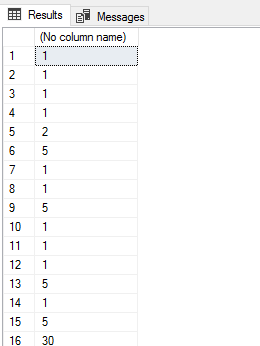
\includegraphics[width=5cm]{./Imagenes/a7a3} 
	\end{center}
	\item Determinar el n\'umero de Administradores o Supervisores utilizar la columna manager\_id para esto. Etiquetar la columna como No de Administradores
	\\	
	\\SELECT COUNT(DISTINCT manager\_id) AS "Numero de Administradores"
	\\FROM employees;
	\begin{center}
	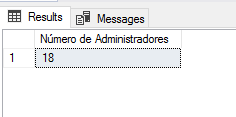
\includegraphics[width=5cm]{./Imagenes/a7a4} 
	\end{center}
	\item Encontrar la diferencia entre el m\'aximo y m\'inimo salario de los empleados. Etiquetar la columna como Diferencia
	\\
	\\SELECT (MAX(salary) - MIN(salary)) AS "diferencia"
	\\FROM employees;
	\begin{center}
	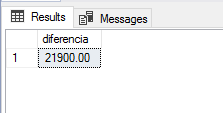
\includegraphics[width=5cm]{./Imagenes/a7a5} 
	\end{center}
	\item Crear un reporte que muestre los No de Administradores (manager\_id) y el salario de su empleado peor pagado. Excluir a los empleados cuyo Administrador no se conozca. Excluir asimismo cualquier grupo cuyo salario mínimo sea \$6000 o menos. Ordenar los resultados por el mínimo salario en forma descendente.
	\\
	\\SELECT salman.minimo,
	\\salman.manager\_id
	\\FROM (SELECT MIN(salary) AS 'minimo',
	\\manager\_id
	\\FROM employees
	\\WHERE salary>6000
	\\GROUP BY manager\_id) AS salman
	\\ORDER BY salman.minimo;
	\begin{center}
	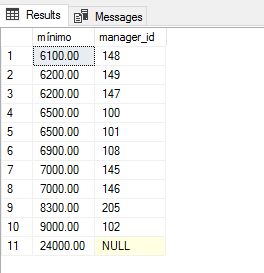
\includegraphics[width=5cm]{./Imagenes/a7a6} 
	\end{center}
	\item Crear una consulta que muestre el número total de empleados, así como el número total de empleados contratados en los años 1995, 1996, 1997 y 1998, etiquetar las columnas apropiadamente.
	\item Crear una consulta matriz que muestre el puesto, el salario por cada puesto basado en el No de Departamento del empleado y el total del salario para cada puesto para los departamento 20, 50, 80 y 90, colocar un nombre apropiado a cada columna.
\end{enumerate}

